\chapter{\texorpdfstring{\MakeUppercase{Simplified Example}}{Simplified Example}}

This chapter serves to show a simplified example of the optimization of
the supply air temperature under one given condition. The single example
is studied in detail in order to present the various competing concerns
impacting the total power required to satisfy the building loads. 

For simplicity, a single duct variable air volume system with two
terminal units is assumed. Hot and dry outdoor air conditions are
assumed such that both zones are under a cooling load and there are no
latent load concerns.  

Zone 1 is assumed to have a load of \SI{20000}{\btu\per\hour}, while the
load in Zone 2 is \SI{7344}{\btu\per\hour}. 

The minimum flow setting for the terminal units is \SI{400}{\cfm}. The
room temperature is \SI{72}{\degreeF} and the mixed air temperature is
\SI{80}{\degreeF}.

The fan is assumed to have the following part-load behavior. The design
flow is chosen so that at a supply temperature of \SI{65}{\degreeF} the
fan is at design flow. 

The design power is chosen so that at the calculated design flow, the
efficiency is \num{0.8} and the pressure rise is \SI{4}{\inchwater}.
Under the chosen conditions, the design flow is \SI{3503}{\cfm}, which
is the resulting flow under the highest tested supply air temperature
\SI{65}{\degreeF}. The resulting design fan power is \SI{2.75}{\hp}. 

\begin{equation}
    \text{FFLP} = A + \left(1-A\right)(\text{PLR})^{n} =   0.1 + (0.9)(\text{PLR})^{2.5}
\end{equation}
The fan power is 
\begin{equation}
    \dot{W}_{fan} = \text{FFLP} \; \dot{W}_{design} = \text{FFLP}\left(\SI{2.75}{\hp}\right) 
\end{equation}

The required flow for each zone is calculated as 
\begin{equation}
    \flow{z} = \text{MAX} \left( \frac{\heatenergy{z}}{C_{a}
    \left(T_{z} - T_{sa}\right)  }, \flow{min}  \right)
\end{equation}
The discharge temperature for each zone is
\begin{equation}
    T_{dis} = T_{z} - \frac{\heatenergy{z}}{C_{a} \; \flow{z}}
\end{equation}
The reheat power is 
\begin{equation}
    \heatenergy{reheat} = C_{a} \flow{z} \left(T_{dis} - T_{sa}\right)
\end{equation} 
and the sensible cooling power is 
\begin{equation}\label{eq:sensibleCoolingPower}
    \heatenergy{cool} = C_{a} \flow{tot} \left(T_{ma} - T_{sa}\right)
\end{equation} 
where \(\flow{tot}\) is the total flow for all the zones. 


\begin{table}
\centering
\caption{Summary of parameters used for simplified example.}
\label{tab:summaryOfParametersForSimplifiedExample}
\begin{tabular}{rl}\toprule
    Parameter              & Value                     \\ \midrule
  System Type              & SDVAV                     \\
  Mixed air temperature    & \SI{80}{\degreeF}         \\
  Zone temperature         & \SI{72}{\degreeF}         \\
  Zone 1 Cooling Load      & \SI{20000}{\btu\per\hour} \\
  Zone 2 Cooling Load      & \SI{7344}{\btu\per\hour}  \\
  Design fan efficiency    & 0.80                      \\
  Design fan pressure rise & \SI{4}{\inchwater}        \\
  Design fan power         & \SI{2.75}{\hp}            \\
  Fan exponent, \(n\)      & 2.5                       \\
  \bottomrule
\end{tabular}
\end{table}

Increasing the supply air temperature has the effect of decreasing
reheat and increasing fan power. Whether the cooling load increases or
decreases depends on several factors. 

For example, during times when there is no reheat, the required flow for
the terminal units is 
\begin{equation}\label{eq:requiredFlow}
    \flow{req} = \frac{\heatenergy{z}}{C_{a} \left(T_{z} - T_{sa}\right)}
\end{equation}
%
Substituting \eqreftext{} \ref{eq:requiredFlow} into  
\eqreftext{} \ref{eq:sensibleCoolingPower} results in
%
\begin{equation}
    \heatenergy{cool} = C_{a}  \frac{\heatenergy{z}}{C_{a} \left(T_{z} -
    T_{sa}\right)}\left(T_{ma} - T_{sa}\right) = \heatenergy{z}
    \frac{T_{ma} - T_{sa}}{T_{z} - T_{sa}}
\end{equation}


What is of interest is how the sensible cooling power is impacted when
the supply air temperature is increased. To investigate, the derivative
of the sensible cooling power equation is found.

\begin{equation}\label{eq:derivativeOfSensibleCooling}
    \dv{\heatenergy{cool}}{T_{sa}} = \heatenergy{z} \frac{T_{ma} -
    T_{z}}{\left(T_{z} - T_{sa}\right)^{2}}
\end{equation}

What \eqreftext{} \ref{eq:derivativeOfSensibleCooling} shows is the
non-intuitive result that during times of cooling, corresponding to a
positive \(\heatenergy{z}\), and when the mixed air temperature is
greater than the zone temperature, corresponding to a positive value in
the numerator of \eqreftext{} \ref{eq:derivativeOfSensibleCooling}, that
the sensible cooling power \textit{increases} with increasing supply air
temperature. If a cooling load exists and the mixed air temperature is
less than the zone temperature, then the opposite is true, increasing
the supply air temperature will reduce the required sensible cooling
power.

\figref{} \ref{fig:simplifiedExampleFlow} shows how the supply air flow
changes with regards to the supply air temperature. The zone loads were
chosen in such a way that Zone 1 operates above the minimum flow
setpoint at all times, while Zone 2 is at the minimum flow setpoint at
supply air temperatures less than \SI{57}{\degreeF}. The system uses
reheat at supply air temperatures less than \SI{57}{\degreeF}. 

With the selected system parameters, the total steady state power can be
plotted with respect to the supply air temperature. The total power
function ends up being convex with a minimum at \SI{57}{\degreeF}. 

What is important is the fact that the optimum supply air temperature is
not simply the maximum supply air temperature in the search range. Under
conditions such as the one in the first example, there is a competing
balance between the cooling, reheat, and fan power. It is possible that
the optimization will potentially suggest lowering the supply air
temperature when the conditions are appropriate.

This conclusion is affirmed as well after investigating the impact of
energy cost. The following analysis assumes the fan power is met by
electricity, the cooling is from district chilled water, and the reheat
is from district hot water, and the prices are those from the posted
Texas A\&M Utilities and Energy Services rates for
FY2016\footnote{https://utilities.tamu.edu/2015/08/31/cost-and-fees-for-utility-services-fy2016/}
The rates are 

\begin{itemize}
    \item Electricity -- \$0.082/kWh
    \item Chilled Water -- \$15.25/MMBTU
    \item Hot Water -- \$15.03/MMBTU
\end{itemize}

When the cost of electricity is taken into account, the importance of
the relationship between fan power and the supply air temperature is
increased. Chilled water is usually produced with a chiller having a COP
greater than 3 while the electricity is consumed directly for the fan.
When the impact of cost is added, the cost penalty for fan power grow
significantly at higher supply air temperatures, which can be seen in
\figref{} \ref{fig:simplifiedExampleCost}. 

With cost as the optimization function, the optimal supply air
temperature is reduced from \SI{57}{\degF} to \SI{49.6}{\degF}. However,
the slope of the total cost curve is flat for supply air temperatures
between \SI{45}{\degF} and \SI{55}{\degF} and any of those temperatures
would be adequate for this particular example. 

% Plots/33-SimplifiedExampleFlow/simplifiedExampleFlow.tex
\begin{figure}
\centering
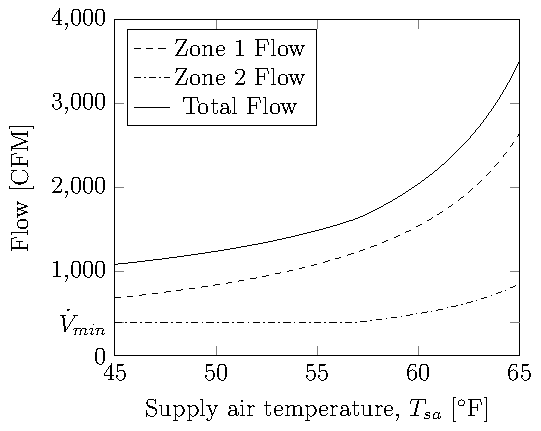
\includegraphics{Plots/33-SimplifiedExampleFlow/simplifiedExampleFlow.pdf}
\caption{Variation of required air flow with respect to different supply
air temperatures.}
\label{fig:simplifiedExampleFlow}
\end{figure}

\newcommand{\variationCaption}[1]{Variation of total #1 with respect to different supply air temperatures. }

\begin{figure}
\centering
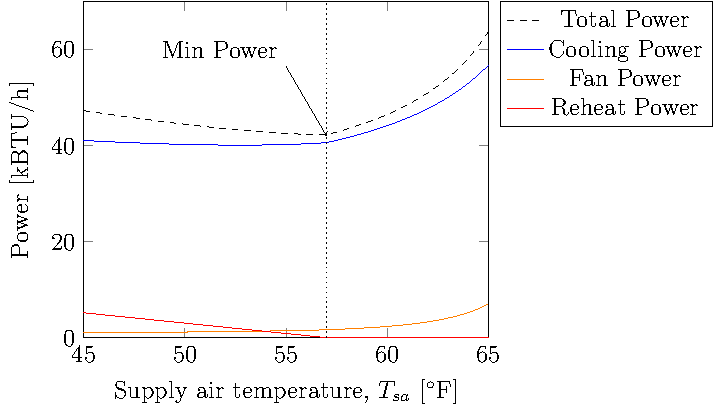
\includegraphics{Plots/32-SimplifiedExample/simplifiedExample.pdf}
\caption{\variationCaption{power}}
\label{fig:simplifiedExamplePower}
\end{figure}

\begin{figure}
\centering
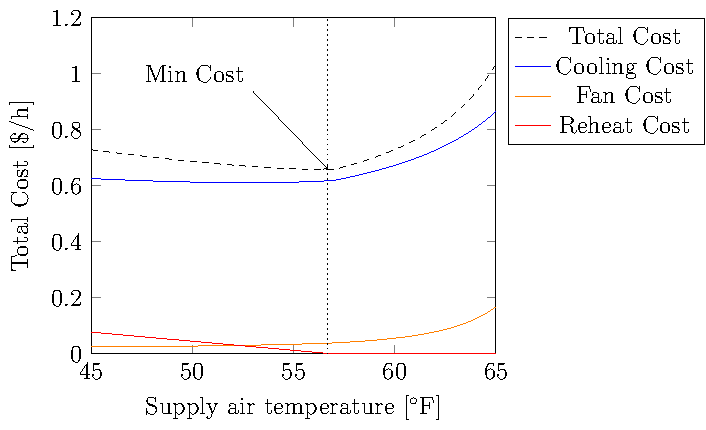
\includegraphics{Plots/35-SimplifiedExampleCostHighMAT/simplifiedExampleCostHighMAT.pdf}
\caption{\variationCaption{cost}}
\label{fig:simplifiedExampleCost}
\end{figure}


If the mixed air temperature is reduced from \SI{80}{\degreeF} to
\SI{65}{\degreeF}, the resulting total power function changes
drastically. The required flow rates for each of the zones remains the
same, along with the fan power and the reheat power. Since the mixed air
temperature is less than the zone temperature, the slope of the sensible
cooling power function is always negative, since the numerator in
\eqreftext{} \ref{eq:derivativeOfSensibleCooling} is negative. The
result of this is that the minimum total power occurs at the maximum of
the supply air temperature search range.   

The optimal supply temperature changes drastically when the cost
differences between electricity and district chilled and hot water is
considered. The lowest power occurs at the highest supply air
temperature, while the lowest cost occurs at \SI{55.4}{\degreeF}. 

\newcommand{\variationCaptionLowMAT}[1]{Variation of total #1 with respect to different supply air
temperatures, with a mixed air temperature of \SI{65}{\degreeF} instead
of the original \SI{80}{\degreeF}.}

\begin{figure}
\centering
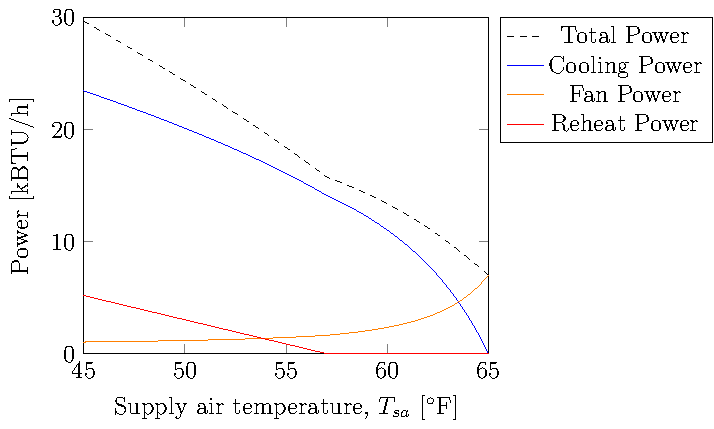
\includegraphics{Plots/34-SimplifiedExampleLowerMAT/simplifiedExampleLowerMAT.pdf}
\caption{\variationCaptionLowMAT{power}}
\label{fig:simplifiedExamplePowerLowerMAT}
\end{figure}

\begin{figure}
\centering
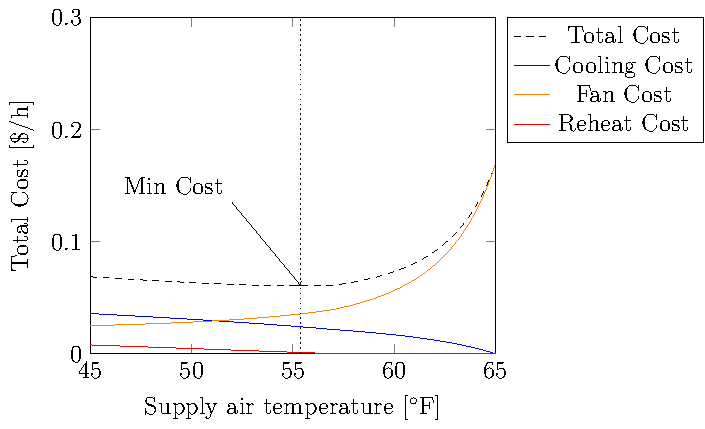
\includegraphics{Plots/36-SimplifiedExampleCostLowerMAT/simplifiedExampleCostHighMAT.pdf}
\caption{\variationCaptionLowMAT{cost}}
\label{fig:simplifiedExampleCostLowerMAT}
\end{figure}



